\section{Apresentação}

\begin{frame} % Capa
    \titlepage
\end{frame}

\begin{frame}{Apresentação}
    \begin{itemize}
        \item Professor {\fontfamily{augie}\selectfont Rodrigo de Farias Gomes}
        \item Telefone (somente mensagens): (92) 9 9405-1724
        \item E-mail: shpnft@gmail.com

    \end{itemize}

    \centering

    \vspace{2cm}
    \begin{tabular}{cccccc}
        R & G & O & M & E & S \\ \\
        \(\color{red} \left.\phantom{{\scriptstyle +1}\frac{1}{2}}\right\downarrow {\scriptstyle +1}~~\) &
        \(\color{red} \left.\phantom{{\scriptstyle +1}\frac{1}{2}}\right\downarrow {\scriptstyle +1}~~\) &
        \(\color{red} \left.\phantom{{\scriptstyle +1}\frac{1}{2}}\right\downarrow {\scriptstyle +1}~~\) &
        \(\color{red} \left.\phantom{{\scriptstyle +1}\frac{1}{2}}\right\downarrow {\scriptstyle +1}~~\) &
        \(\color{red} \left.\phantom{{\scriptstyle +1}\frac{1}{2}}\right\downarrow {\scriptstyle +1}~~\) &
        \(\color{red} \left.\phantom{{\scriptstyle +1}\frac{1}{2}}\right\downarrow {\scriptstyle +1}~~\) \\ \\
        S & H & P & N & F & T
    \end{tabular}
\end{frame}

\begin{frame}{Calendário}
    \centering
    \small{
        \begin{tabular}{cP{2cm}P{2cm}P{2cm}P{2cm}P{2cm}}
            \rowcolor{black!10} & Segunda & Terça & Quarta & Quinta & Sexta \\
            01 & \dma{0} & \dma{1} & \dma{2} & \dma{3} & \dma{4} \\
            02 & \dma{7} & \dma{8} & \dma{9} & \dma{10} & \dma{11} \\
            03 & \dma{14} & \dma{15} & \dma{16} & \dma{17} & \dma{18} \\
            04 & \dma{21} & \dma{22} & \dma{23} & \dma{24} & \dma{25} \\
            05 & \dma{28} & \dma{29} & \dma{30} & \dma{31} & \dma{32} \\
            06 & \dma{35} & \dma{36} & \dma{37} & \dma{38} & \dma{39} \\
            07 & \dma{42} & \dma{43} & \dma{44} & \dma{45} & \dma{46} \\
            08 & \dma{49} & \dma{50} & \dma{51} & \dma{52} & \dma{53} \\
            09 & \dma{56} & \dma{57} & \dma{58} & \dma{59} & \dma{60} \\
            10 & \dma{63} & \dma{64} & \dma{65} & \dma{66} & \dma{67} \\
            11 & \dma{70} & \dma{71} & \dma{72} & \dma{73} & \dma{74} \\
            12 & \dma{77} & \dma{78} & \dma{79} & \dma{80} & \dma{81} \\
            13 & \dma{84} & \dma{85} & \dma{86} & \dma{87} & \dma{88} \\
            14 & \dma{91} & \dma{92} & \dma{93} & \dma{94} & \dma{95} \\
            15 & \dma{98} & \dma{99} & \dma{100} & \dma{101} & \dma{102} \\
            % 16 & \dma{103} & \dma{104} & \dma{105} & \dma{106} & \dma{107} \\
            % 17 & \dma{108} & \dma{109} & \dma{110} & \dma{111} & \dma{112} \\
        \end{tabular}
    }
\end{frame}

\begin{frame}{Meus horários em 20/03/2023...}
    \small{
        \begin{center}
            \begin{tabular}{ccccc}
                \rowcolor{black!10} Segunda & Terça & Quarta & Quinta & Sexta \\ \hline
                \rowcolor{red!25} &&&& \\ \hline
                \rowcolor{red!25} Métodos Num... & Trigonometria & Métodos Num... & Trigonometria & \\ \hline
                \rowcolor{green!25} & & Termodinâmica & & Termodinâmica \\ \hline
                \rowcolor{green!25} & Óptica e Eletro... & & Óptica e Eletro... & \\ \hline
                \rowcolor{blue!25} &&&& \\ \hline
                \rowcolor{blue!25} &&&& \\ \hline
            \end{tabular}
        \end{center}

        \vspace{1cm}
        Legenda:
        \begin{itemize}
            \item[\textcolor{red!25}{\rule{1em}{1em}}] Manhã (8:00 -- 10:00 e 10:00 -- 12:00)
            \item[\textcolor{green!25}{\rule{1em}{1em}}] Tarde (14:00 -- 16:00 e 16:00 -- 18:00)
            \item[\textcolor{blue!25}{\rule{1em}{1em}}] Noite (18:00 -- 20:00 e 20:00 -- 22:00)
        \end{itemize}
    }
\end{frame}

\begin{frame}[label=ementa]{Ementa de \Disciplina}
    \begin{itemize}
        \item Conceitos fundamentais
        \item Equação de estado
        \item Primeira Lei da Termodinâmica
        \item Algumas consequências da Primeira Lei
        \item Entropia e Segunda Lei da Termodinâmica
        \item Primeira e Segunda Leis combinadas
        \item Potenciais termodinâmicos
        \item Aplicações da termodinâmica a sistemas simples
        \item Forças intermoleculares
        \item Física Estatística
        \item Aplicações da Física Estatística a gases e outros sistemas
    \end{itemize}
\end{frame}

\begin{frame}{Avaliação}
    \begin{itemize}
        \item A avaliação será na forma de 3 notas: \(N_1\), \(N_2\) e \(N_3\)
        \item A média dos exercícios escolares (\(MEE\)) será dada por
            \[
                MEE=\frac{N_1+N_2+N_3}{3}
            \]
        \item Se \(MEE \geq 8,0\), então a média final (\(MF\)) será igual à \(MEE\)
        \item Se \(MEE < 8,0\), então
            \[
                MF=\frac{2\times MEE+PF}{3}
            \]
            onde PF é a nota da \textbf{prova final}
        \item Se \(MF \geq 5,0\) e a frequência em sala for maior que 75\%, o aluno está aprovado
        \item Haverá 30 aulas de \SI{2}{horas}, de forma que \textbf{o número máximo de faltas é 8}
    \end{itemize}
\end{frame}

\begin{frame}{Livro}
    \centering
    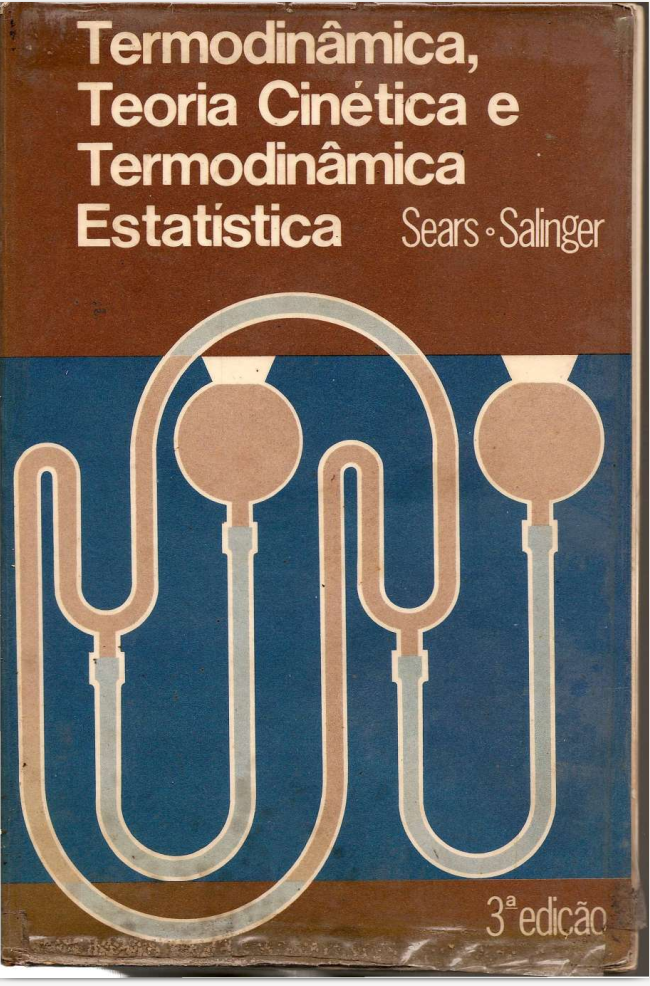
\includegraphics[height=0.8\textheight]{images/Captura de tela de 2023-03-27 07-48-28.png}
\end{frame}

\begin{frame}
    \centering
    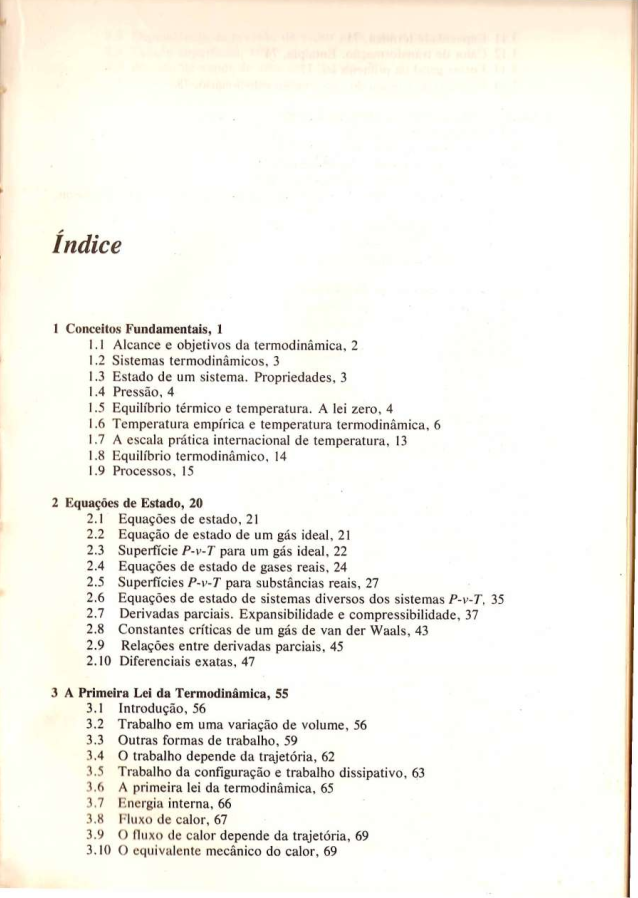
\includegraphics[width=0.32\textwidth]{images/Captura de tela de 2023-03-27 07-48-56.png}
    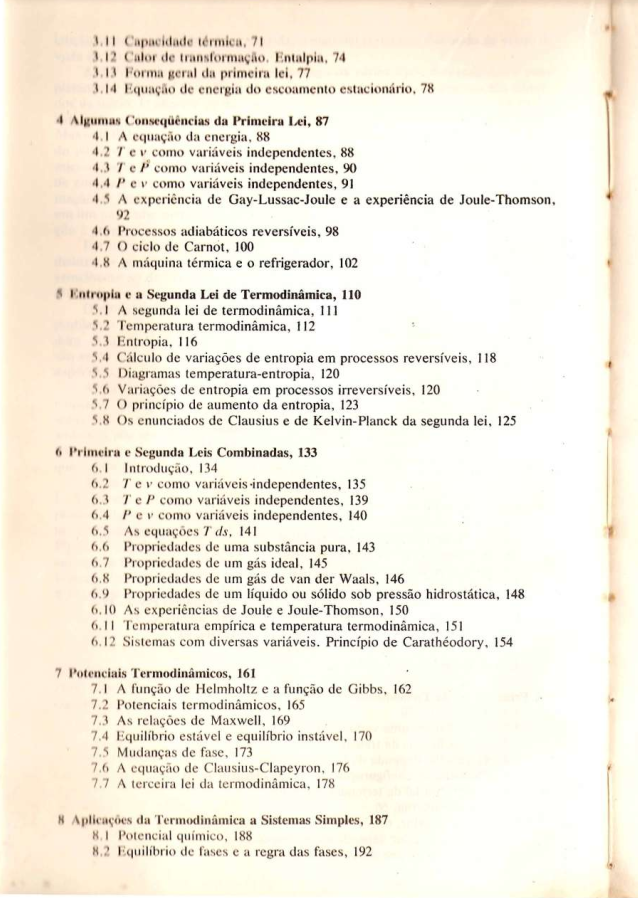
\includegraphics[width=0.32\textwidth]{images/Captura de tela de 2023-03-27 07-49-06.png}
    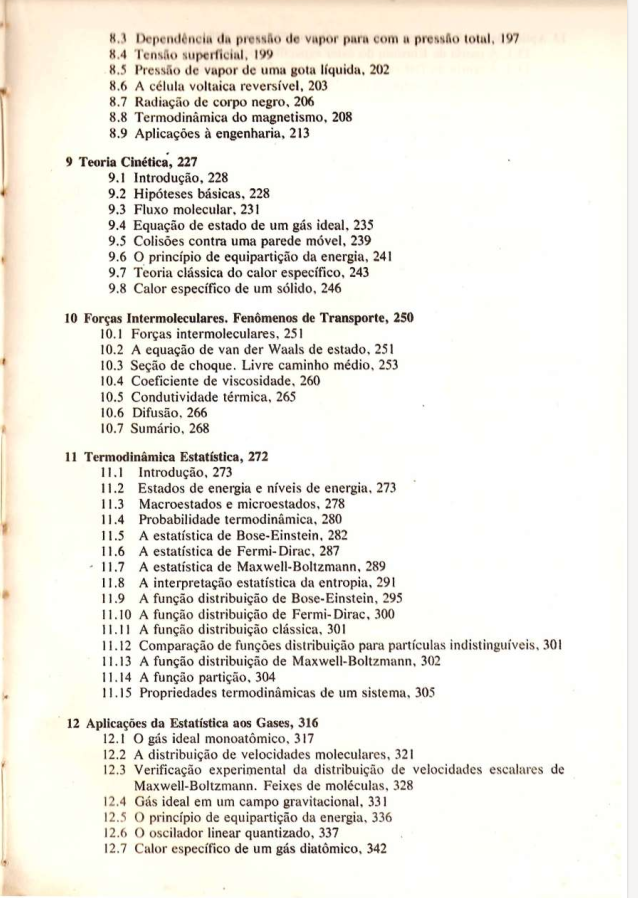
\includegraphics[width=0.32\textwidth]{images/Captura de tela de 2023-03-27 07-49-18.png}
\end{frame}

\againframe<2>{ementa}

\begin{frame}[c]{Termodinâmica}
    \begin{minipage}{\textwidth}
        \color{blue}
        Se as teorias físicas fossem pessoas, a Termodinâmica seria a bruxa da
        aldeia. Ao longo de três séculos, ela sorriu silenciosamente enquanto
        outras teorias surgiam e desapareciam, sobrevivendo a grandes
        revoluções na Física, como o advento da relatividade geral e da
        mecânica quântica. As outras teorias a acham um tanto estranha, de
        alguma forma de natureza diferente do restante, mas todos vêm a ela em
        busca de conselhos e ninguém ousa contradizê-la. Einstein, por exemplo,
        chamou-a de “a única teoria física de conteúdo universal, que estou
        convencido de que dentro da estrutura de aplicabilidade de seus
        conceitos básicos nunca será derrubada”
    \end{minipage}

    \vspace{1cm}
    John Goold \textit{et al} 2016 J. Phys. A: Math. Theor. 49 143001 \\
    https://doi.org/10.1088/1751-8113/49/14/143001
\end{frame}

\begin{frame}[c]{Leis da Termodinâmica, versão poltrona do vovô}
    \begin{itemize}
        \item Lei zero: Se você tocar em alguma coisa, você entra no jogo
        \item Lei um: A vida é um jogo
        \item Lei dois: Você não pode vencer
        \item Lei três: Você não pode nem empatar
    \end{itemize}

    \vspace{1cm}
    Escrito por Thomas Tabb Mayo IV
\end{frame}

\begin{frame}[c]{Mecânica Estatística}
    \begin{minipage}{\textwidth}
        \color{blue}
        Ludwig Boltzmann, who spent much of his life studying statistical
        mechanics, died in 1906, by his own hand. Paul Ehrenfest, carrying on the
        work, died similarly in 1933. Now it is our turn to study statistical
        mechanics.
    \end{minipage}

    \vspace{1cm}
    Texto de David L. Goodstein no livro \textit{States of Matter} (1975)
\end{frame}

\begin{frame}{Então...}
    \begin{itemize}
        \item A Termodinâmica é uma ciência experimental, baseada em um pequeno
            número de princípios, que são generalizações feitas a partir da
            experiência
        \item \textcolor{red}{Ela trabalha apenas com as propriedades \textit{macroscópicas} da
            matéria}
        \item Dos princípios da termodinâmica podemos obter relações gerais
            entre grandezas físicas e como essas dependem da temperatura.
        \item Os princípios da termodinâmica nos dizem quais as relações entre as 
            grandezas físicas que devem ser experimentalmente determinadas para que 
            \textit{todas} as propriedades do sistema sejam \textit{completamente} determinadas
    \end{itemize}
\end{frame}

\begin{frame}{Sistema}
    \begin{itemize}
        \item \textbf{Sistema} é tudo aquilo que queremos estudar. Ele pode ser tão simples 
            como um corpo livre (por exemplo, uma manga caindo de uma árvore) ou tão complexo como
            um motor de combustão
        \item Tudo que é externo ao sistema é considerado parte das \textbf{vizinhanças} do sistema
        \item Um sistema \textbf{fechado} sempre contém a mesma quantidade de matéria, ou seja, 
            não pode ocorrer troca de matéria com a sua vizinhança
        \item Um sistema \textbf{isolado} é um sistema fechado que não interage de forma alguma
            com a sua vizinhança
        \item O \textbf{estado} de um sistema é especificado pelos valores de certas grandezas
            mensuráveis experimentalmente chamadas \textit{variáveis de estado} ou \textit{propriedades}
        \item Exemplos de propriedades são a temperatura, a pressão exercida e o volume ocupado
        \item Note que a energia transferida entre o sistema e sua vizinhança não é uma propriedade
        \item Quando qualquer propriedade de um sistema varia, o estado do sistema varia e diz-se que o 
            sistema está sofrendo um \textbf{processo}
    \end{itemize}
\end{frame}

\begin{frame}{Um processo, dois sistemas...}
    \begin{minipage}{\textwidth}
        Ar está contido em um conjunto cilindro-pistão vertical equipado com uma resistência
        elétrica. A atmosfera exerce uma pressão de \SI{101.3}{kPa} no topo do pistão, que possui
        uma massa de \SI{45.4}{kg} e cuja área da face é de \(\SI{0.09}{m^2}\). Uma corrente 
        elétrica passa através da resistência e o volume aumenta lentamente de \(\SI{0.04}{m^3}\),
        enquanto sua pressão permanece constante. A massa do ar é \SI{0.27}{kg} e sua \textbf{energia interna}
        específica aumenta de \SI{41.9}{kJ/kg}. O ar e o pistão estão em repouso no início e fim do processo.
        O material do cilindro-pistão é um bom isolante. O atrito entre o pistão e a parede do cilindro pode ser 
        desprezado, e a aceleração da gravidade é \(g=\SI{9.7}{m/s^2}\).
    \end{minipage}
    \begin{enumerate}[(a)]
        \item Para um sistema composto de apenas ar, determine a transferência de \textbf{calor} da resistência para o ar 
            e o \textbf{trabalho} realizado \textit{pelo} sistema
        \item Para um sistema composto de ar e pistão, determine a transferência de calor da resistência para o ar 
            e o trabalho realizado pelo sistema
    \end{enumerate}

    \pause

    \begin{tcolorbox}[colback=red!20]
        O que é energia interna, calor e trabalho? Como essas grandezas se relacionam?
    \end{tcolorbox}
\end{frame}

\begin{frame}[c]
    \centering
    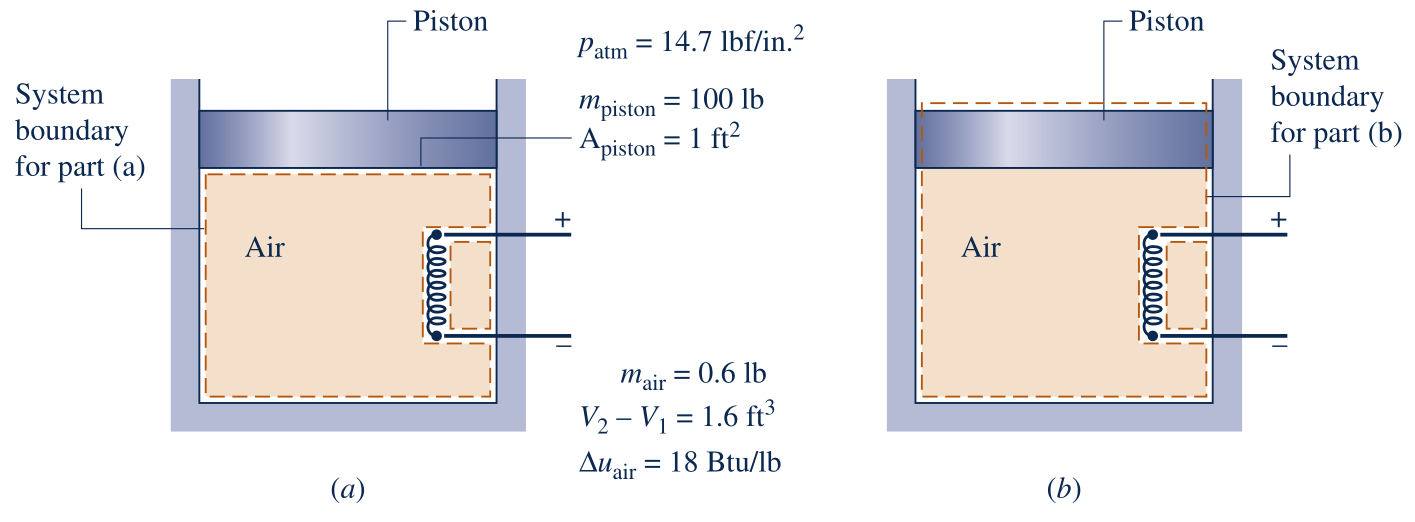
\includegraphics[width=0.9\textwidth]{images/Captura de tela de 2023-03-29 08-03-41.png}
\end{frame}

\begin{frame}{Observações}
    \begin{itemize}
        \item Uma grandeza é uma propriedade se, e somente se, sua mudança de valor
            entre dois estados é independente do processo
        \item Ou seja, se o valor de uma determinada grandeza depende dos detalhes do
            processo e não apenas dos estados extremos, essa grandeza não pode ser uma propriedade
        \item Um sistema está em \textbf{equilíbrio} quando não há mudanças no valor de suas propriedades 
            \textit{após ser isolado}
    \end{itemize}
    \centering
    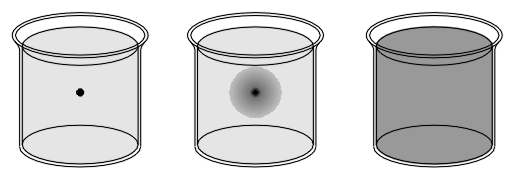
\includegraphics[width=0.8\textwidth]{images/termo4.png}
\end{frame}

\begin{frame}{Pergunta difícil}
    \begin{minipage}{\textwidth}
        Uma mistura de hidrogênio e oxigênio é isolada e deixada alcançar um estado de temperatura 
        e pressão constantes. A mistura é explodida com uma centelha de energia desprezível e novamente
        deixada atingir um estado de temperatura e pressão constantes
    \end{minipage}
    \begin{enumerate}
        \item O estado inicial é um estado de equilíbrio? Explique
        \item O estado final é um estado de equilíbrio? Explique
    \end{enumerate}
\end{frame}

\begin{frame}{Princípio dos estados equivalentes}
\begin{itemize}
    \item Existe uma propriedade \textit{intensiva} independente para cada forma pela qual a energia de um sistema pode ser variada independentemente 
    \item Formas de transferência de energia: calor + trabalho (várias formas)
    \item Ou seja: o número de propriedades \textit{intensiva} independentes é igual  ao número de interações relevantes do sistema devido a trabalho mais um (calor)
\end{itemize}
\begin{block}
    {Sistema compressível simples}
    \begin{itemize}
        \item \textbf{Sistema simples}: existe somente uma forma pela qual a energia do sistema pode ser significativamente alterada por trabalho
        \item \textbf{Sistema compressível simples}: o trabalho é relacionado a uma mudança no volume
        \item Em um sistema compressível simples, a temperatura e o volume específico podem ser considerados independentes e a pressão como função destes dois, ou seja, 
        \(
        P= P(T,v)
        \)
        \item Dessa função temos uma superfície \(P-v-T\)
    \end{itemize}
\end{block}
\end{frame}

\begin{frame}{Superfície P-v-T da água\footnote{possivelmente}}
\centering
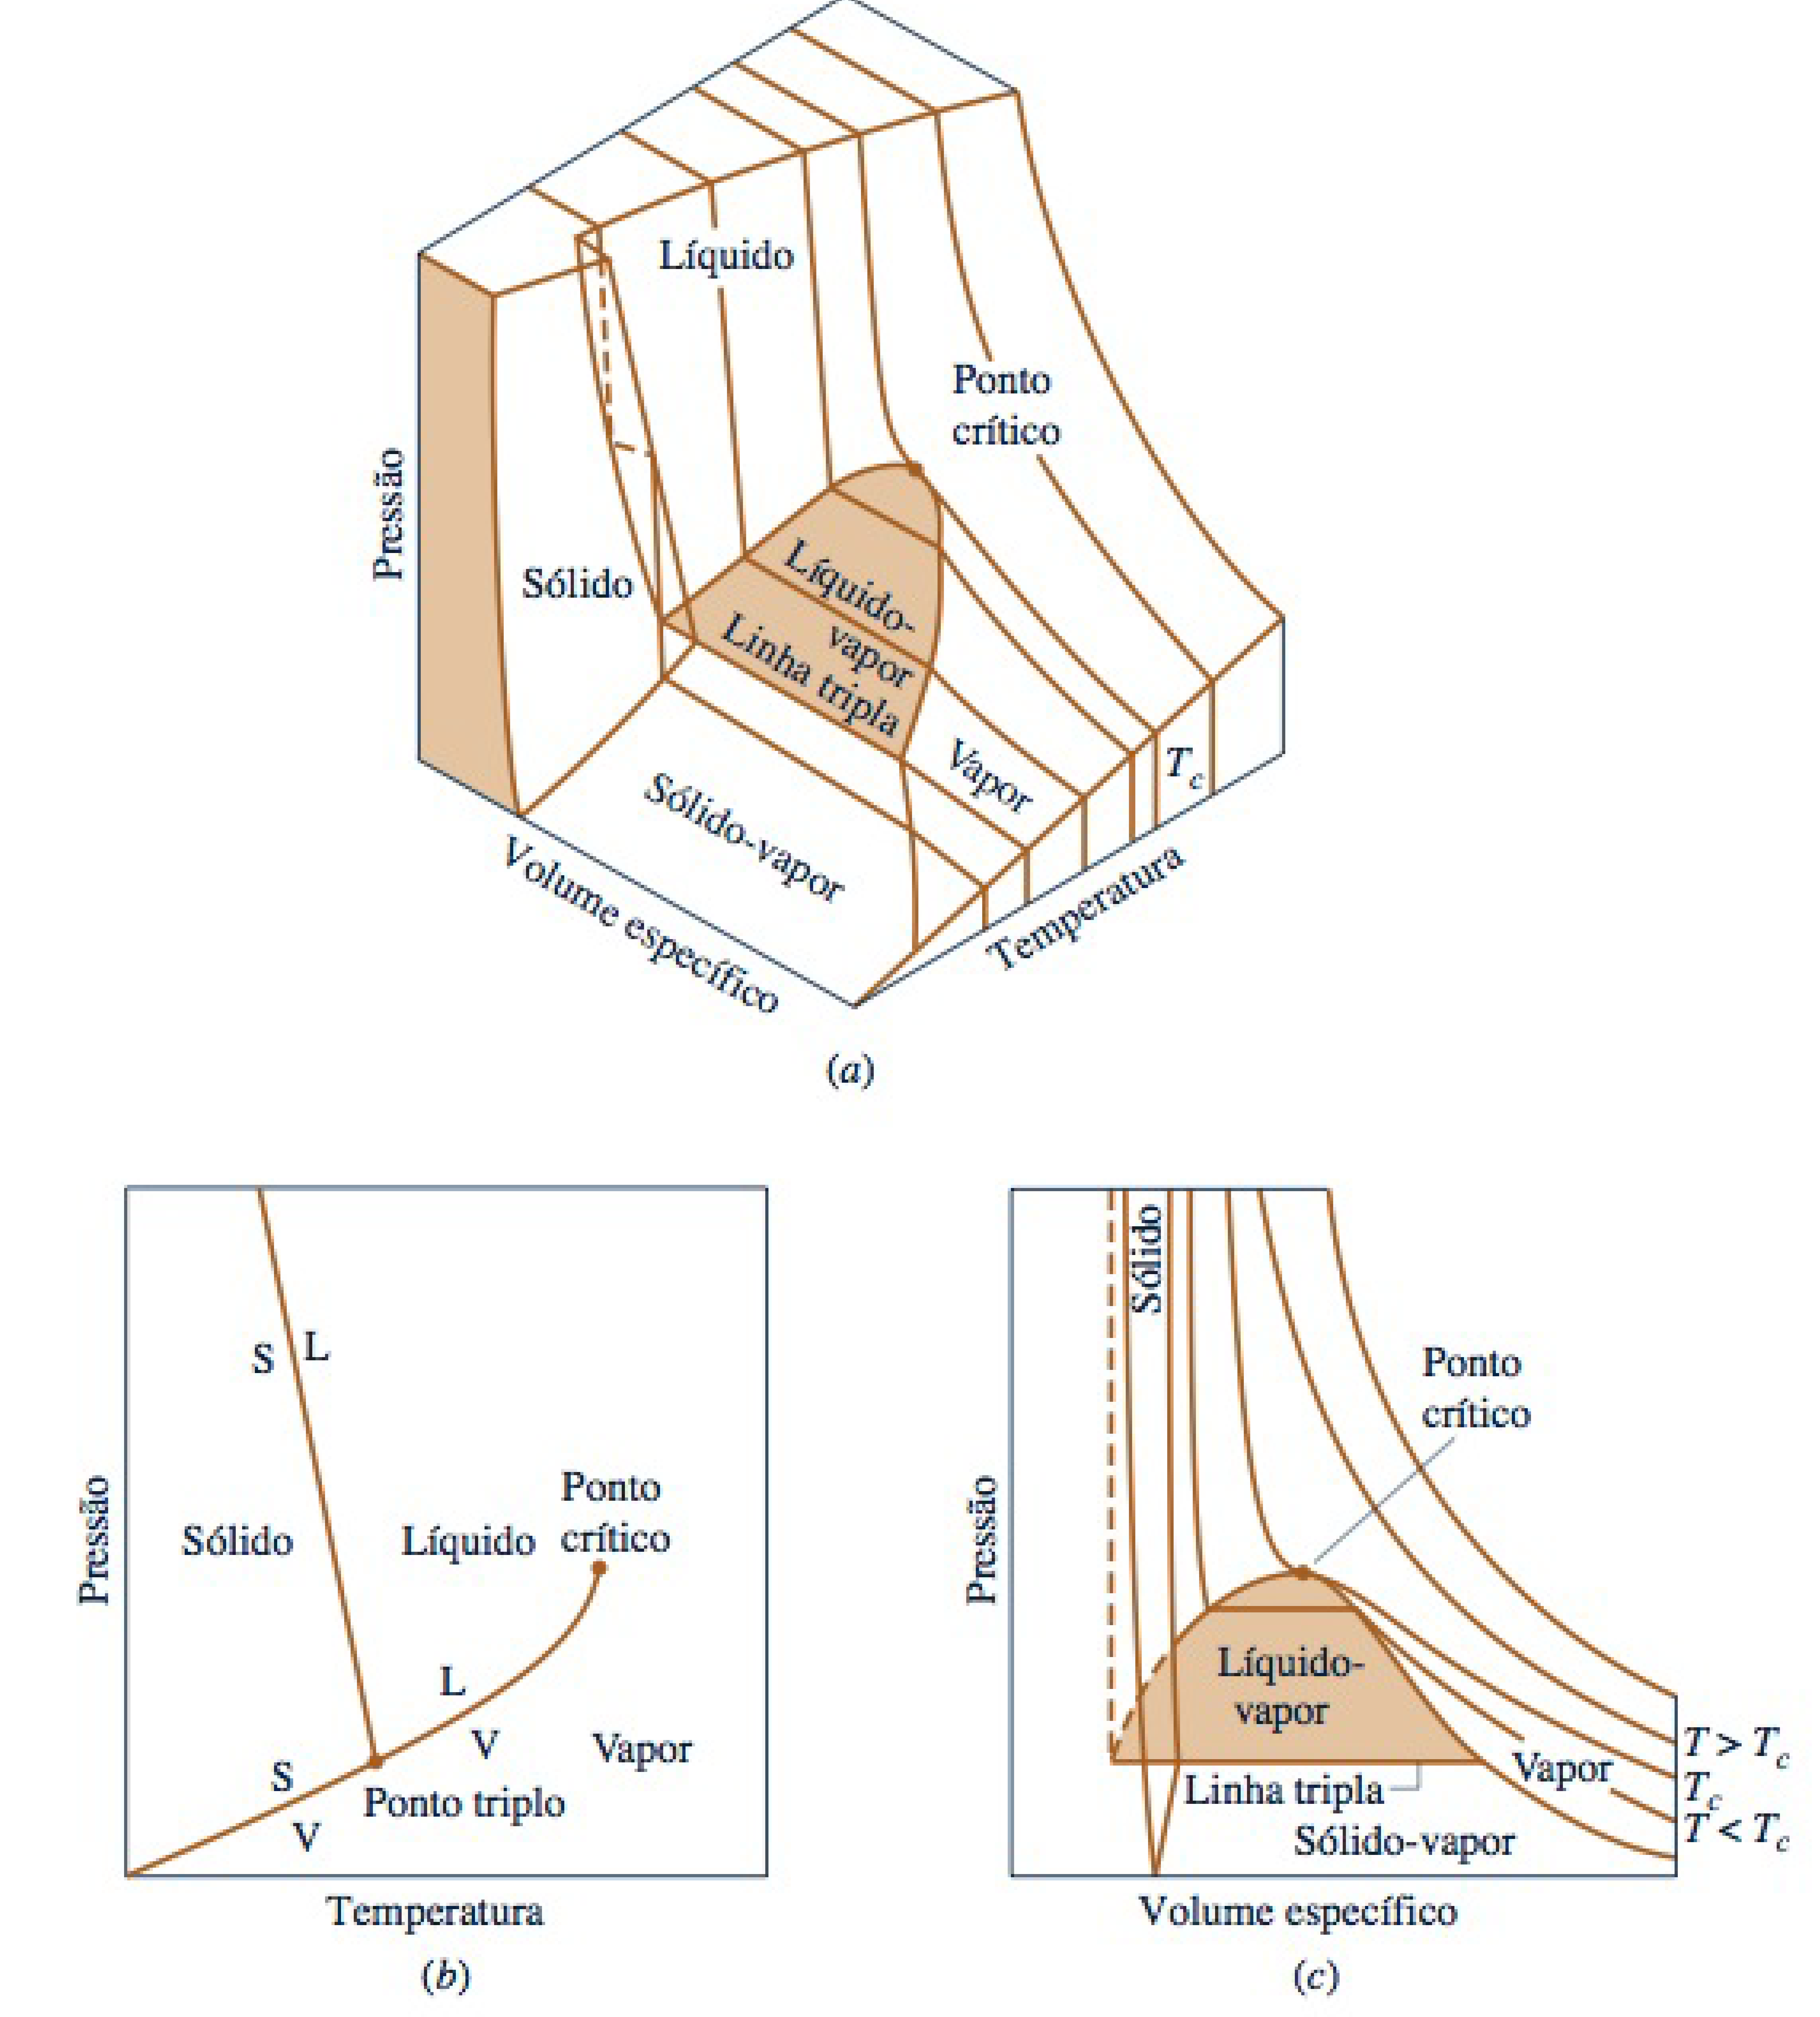
\includegraphics[height=7.5cm-5pt]{images/pvt.png}
\end{frame}

\begin{frame}{Gás ideal}
\[
    Pv = RT \leftarrow \text{equação de estado}
\]
\centering
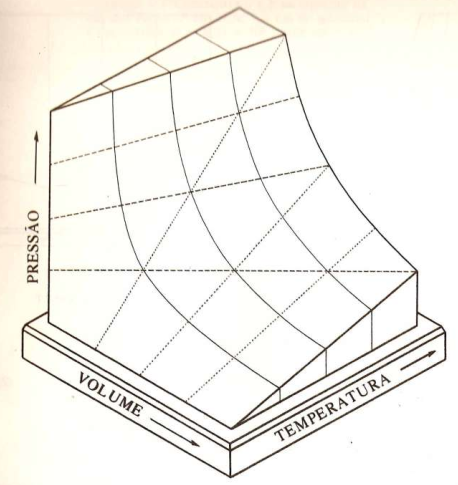
\includegraphics[height=7.5cm-60pt]{images/pvt-ideal.png}

\pause

\(R=\SI{8.3143e3}{\dfrac{J}{kmol~K}}\) é a constante \textbf{universal} dos gases 
\end{frame}

\begin{frame}
    \centering
    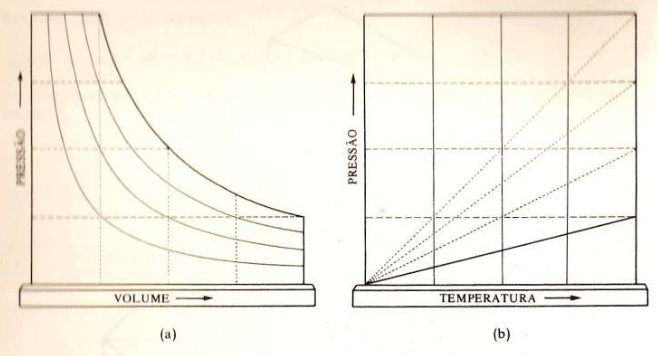
\includegraphics[height=0.8\textheight]{images/Captura de tela de 2023-04-03 13-42-22.png}
    \begin{columns}
        \begin{column}{0.4\textwidth}
            \[
                \textcolor{blue}{P}=R\frac{T}{\textcolor{red}{v}}
            \]
        \end{column}

        \begin{column}{0.4\textwidth}
            \[
                \textcolor{blue}{P}=R\frac{\textcolor{red}{T}}{v}
            \]
        \end{column}
    \end{columns}
\end{frame}

\begin{frame}[c]{Gases de van der Waals}
\[
    \left(P+\frac{a}{v^2}\right)(v-b)=RT
\]

\centering
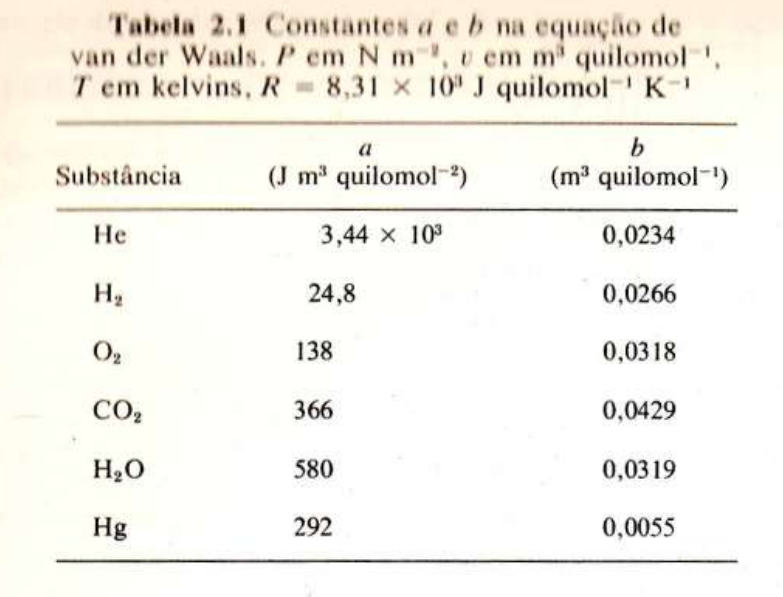
\includegraphics[height=\textheight-70pt]{images/Captura de tela de 2023-04-12 07-51-46.png}
\end{frame}

\begin{frame}[c]
    \begin{columns}[T]
        \begin{column}{0.4\textwidth}
            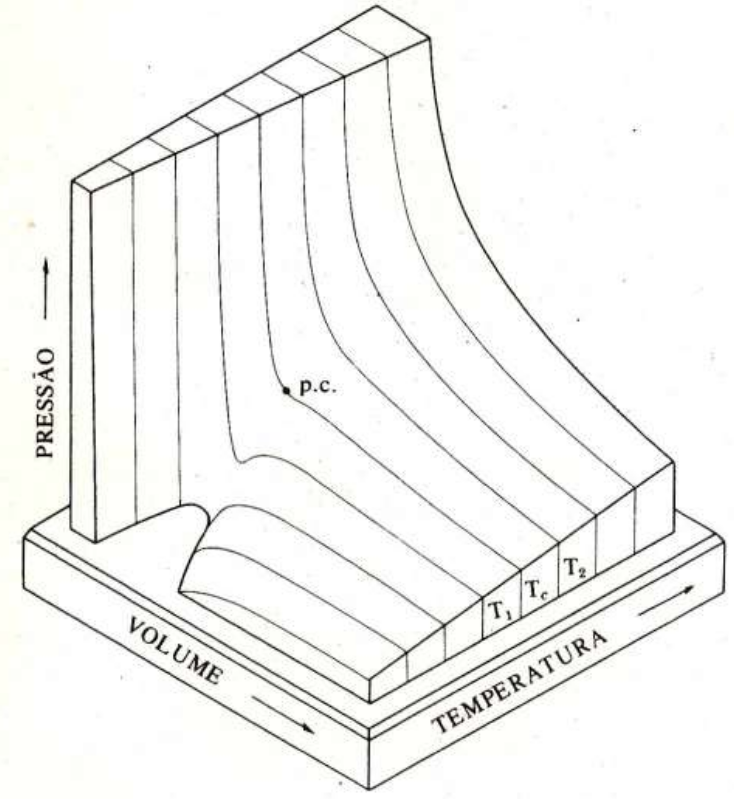
\includegraphics[width=\textwidth]{images/Captura de tela de 2023-04-12 08-15-26.png}
        \end{column}

        \begin{column}{0.4\textwidth}
            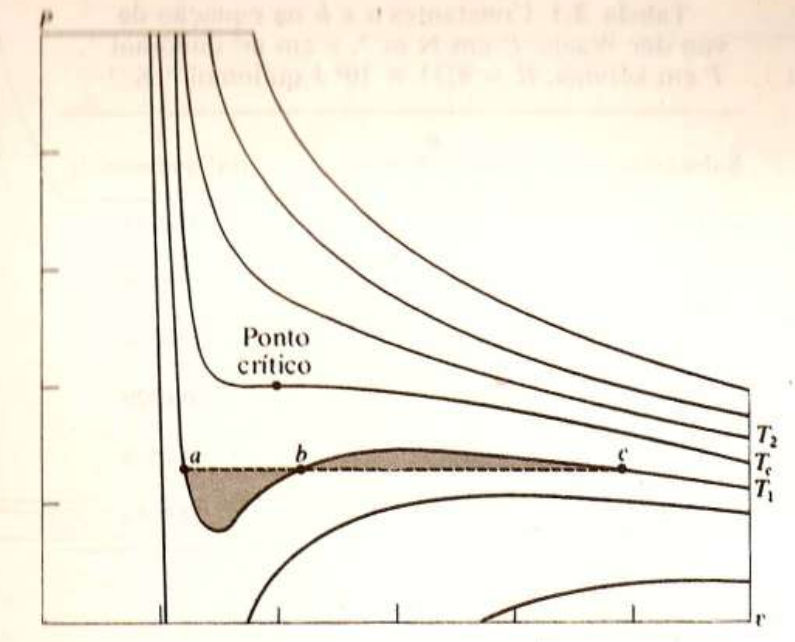
\includegraphics[width=\textwidth]{images/Captura de tela de 2023-04-12 08-17-41.png}
        \end{column}
    \end{columns}
    \pause
    O \textit{ponto crítico} \(pc\) é o ponto \((P,v,T)\) onde as \textit{fases} líquida e gasosa/vapor podem coexistir
\end{frame}

% \begin{frame}{Substância real: \(\text{CO}_2\)}
%     \begin{center}
%         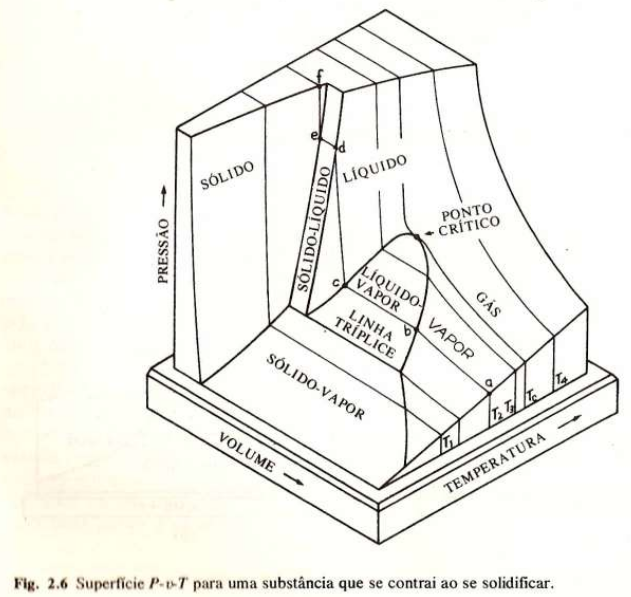
\includegraphics[height=\textheight-35pt]{images/Captura de tela de 2023-04-12 08-40-12.png}
%     \end{center}
% \end{frame}

\begin{frame}[c]{Equação de estado para um fio sob tensão}
    \[
        L=L_0 \left[ 1+ \frac{\mathcal{F}}{YA}+\alpha (T-T_0) \right]
    \]
    onde 
    \begin{itemize}
        \item \(L\) é o comprimento do fio
        \item \(L_0\) é o comprimento sob tensão nula à temperatura \(T_0\)
        \item \(Y\) é o módulo de Young (\textit{propriedade relacionada a elasticidade})
        \item \(A\) é a área da seção reta
        \item \(\alpha\) é o coeficiente de dilatação linear
        \item \(\mathcal{F}\) é a tensão
    \end{itemize}
\end{frame}

\begin{frame}{Cálculo...}
    \begin{itemize}
        \item A equação de estado de um sistema \(PVT\)\footnote{\(v\) e \(V\) são diferentes, por quê?} 
            é uma relação entre \(P\), \(V\) e \(T\) em qualquer estado de equilíbrio do sistema
        \item Há muitas outras propriedades no sistema e, possivelmente, outras equações de estado
        \item O \textit{coeficiente de dilatação volumétrica} de um material é definido como
            \[
                \beta \equiv \frac{1}{V}\left(\frac{\partial V}{\partial T}\right)_P
            \]
        \item O \textit{coeficiente de compressão isotérmica} de um material é definido como
            \[
                \kappa \equiv -\frac{1}{V}\left(\frac{\partial V}{\partial P}\right)_T
            \]
        \item Como vimos em Cálculo, se \(V\)\footnote{na verdade, \(v\)...} é uma propriedade e \(V=V(P,T)\), temos
            \[
                dV = \frac{\partial V}{\partial T} dT + \frac{\partial V}{\partial P} dP 
                \implies dv = \beta V dT - \kappa V dP
            \]
    \end{itemize}
\end{frame}

\begin{frame}
    \begin{itemize}
        \item Se a equação anterior for integrada de algum estado de referência
            \(V_0\), \(P_0\), \(T_0\) até algum estado arbitrário
            \(V\), \(P\), \(T\) obteremos
            \[
                \int_{V_0}^V = V-V_0 = \int_{T_0}^T \beta V dT
                - \int_{P_0}^P \kappa V dP
            \]
        \item \textcolor{red}{Considerando} \(V\) constante  quando \(P\) e \(T\)
            são variadas e, além disso, \(\beta\) e \(\kappa\) também
            constantes, temos que
            \[
                V=V_0 [ 1+\beta (T-T_0) - \kappa (P-P_0)]
            \]
            \textcolor{red}{ou seja, é possível obter a equação de estado de um sólido ou líquido}
    \end{itemize}
\end{frame}
